% This file was created with tikzplotlib v0.9.15.
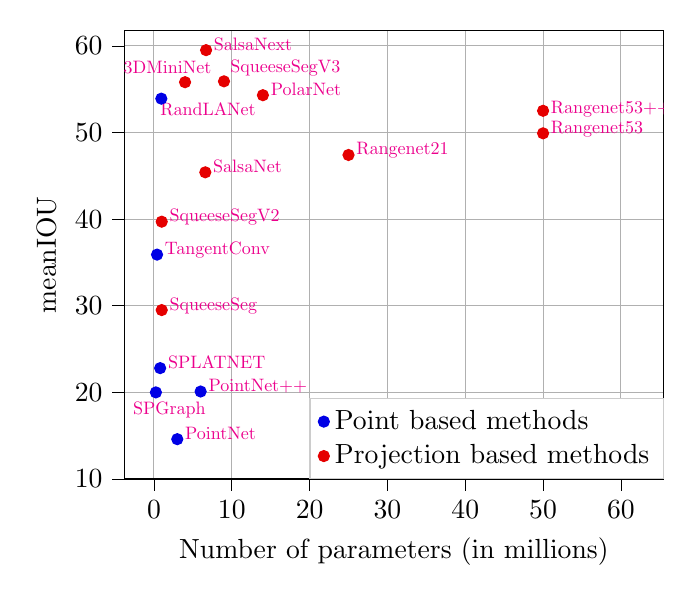
\begin{tikzpicture}

  \definecolor{blue0}{rgb}{0, 0, 0.9}
  \definecolor{red0}{rgb}{0.9, 0, 0}
  
  \begin{axis}[
  legend cell align={left},
  legend style={fill opacity=1, draw opacity=1, text opacity=1, at={(1,0.18)}, draw=white!80!black},
  tick align=outside,
  tick pos=left,
  x grid style={white!69.0196078431373!black},
  xlabel={Number of parameters (in millions)},
  xmajorgrids,
  xmin=-3.8375, xmax=65.5,
  xtick style={color=black},
  y grid style={white!69.0196078431373!black},
  ylabel={meanIOU},
  ymajorgrids,
  ymin=10, ymax=61.745,
  ytick style={color=black}
  ]
  
  \addplot[draw=blue0, fill=blue0, mark=*, only marks, mark size=2pt]
  table{
  x y
  3 14.6
  6 20.1
  0.25 20
  0.8 22.8
  0.4 35.9
  0.95 53.9
  };
  \addlegendentry{Point based methods}
  \addplot[draw=red0, fill=red0, mark=*, only marks, mark size=2pt]
  table{
  x y
  1 29.5
  1 39.7
  4 55.8
  6.7 59.5
  6.6 45.4
  25 47.4
  50 49.9
  50 52.5
  14 54.3
  9 55.9
  };
  \addlegendentry{Projection based methods}
  \draw (axis cs:1.2,29.5) node[
    scale=0.65,
    anchor=base west,
    text=magenta,
    rotate=0.0
  ]{SqueeseSeg};
  \draw (axis cs:1.2,39.7) node[
    scale=0.65,
    anchor=base west,
    text=magenta,
    rotate=0.0
  ]{SqueeseSegV2};
  \draw (axis cs:9,56.9) node[
    scale=0.65,
    anchor=base west,
    text=magenta,
    rotate=0.0
  ]{SqueeseSegV3};
  \draw (axis cs:8.2,56.8) node[
    scale=0.65,
    anchor=base east,
    text=magenta,
    rotate=0.0
  ]{3DMiniNet};
  \draw (axis cs:6.9,59.5) node[
    scale=0.65,
    anchor=base west,
    text=magenta,
    rotate=0.0
  ]{SalsaNext};
  \draw (axis cs:6.8,45.4) node[
    scale=0.65,
    anchor=base west,
    text=magenta,
    rotate=0.0
  ]{SalsaNet};
  \draw (axis cs:25.2,47.4) node[
    scale=0.65,
    anchor=base west,
    text=magenta,
    rotate=0.0
  ]{Rangenet21};
  \draw (axis cs:50.2,49.9) node[
    scale=0.65,
    anchor=base west,
    text=magenta,
    rotate=0.0
  ]{Rangenet53};
  \draw (axis cs:50.2,52.2) node[
    scale=0.65,
    anchor=base west,
    text=magenta,
    rotate=0.0
  ]{Rangenet53++};
  \draw (axis cs:3.2,14.6) node[
    scale=0.65,
    anchor=base west,
    text=magenta,
    rotate=0.0
  ]{PointNet};
  \draw (axis cs:6.2,20.1) node[
    scale=0.65,
    anchor=base west,
    text=magenta,
    rotate=0.0
  ]{PointNet++};
  \draw (axis cs:7.45,17.5) node[
    scale=0.65,
    anchor=base east,
    text=magenta,
    rotate=0.0
  ]{SPGraph};
  \draw (axis cs:1,22.8) node[
    scale=0.65,
    anchor=base west,
    text=magenta,
    rotate=0.0
  ]{SPLATNET};
  \draw (axis cs:0.6,35.9) node[
    scale=0.65,
    anchor=base west,
    text=magenta,
    rotate=0.0
  ]{TangentConv};
  \draw (axis cs:0,51.9) node[
    scale=0.65,
    anchor=base west,
    text=magenta,
    rotate=0.0
  ]{RandLANet};
  \draw (axis cs:14.2,54.3) node[
    scale=0.65,
    anchor=base west,
    text=magenta,
    rotate=0.0
  ]{PolarNet};
  \end{axis}
  
  \end{tikzpicture}
  